%------------------------------------------------------------------------
% Chapter:  Introduction
%------------------------------------------------------------------------

\chapter{Example refinements \label{example}}

The example in this chapter will be used to explain in detail the 
commands and control variables that \Diffev uses. The example is a 
simple function y = F(x). While this restriction eases the display of the 
data, and refinement process, it does not impose a restriction on the
settings.

The macros and input data needed to run this example are found along
with the \Diffev source code, in the directory {\em diffev/TESTS}.

\section{Nanoparticle refinement}

In this section  a full blown refinement of a disordered nanoparticle 
structure is illustrated, which is also to be found in the DISCUS 
book, \cite{nedpro}. The data for the nanoparticle are taken from
\cite{neder2007}. The nanoparticle sample consists of ZnSe nanoparticles.
The PDF was derived from X-ray powder diffraction data taken at beam line 
BW5 at the former storage ring DORIS at DESY, Germany. 

\begin{figure}
   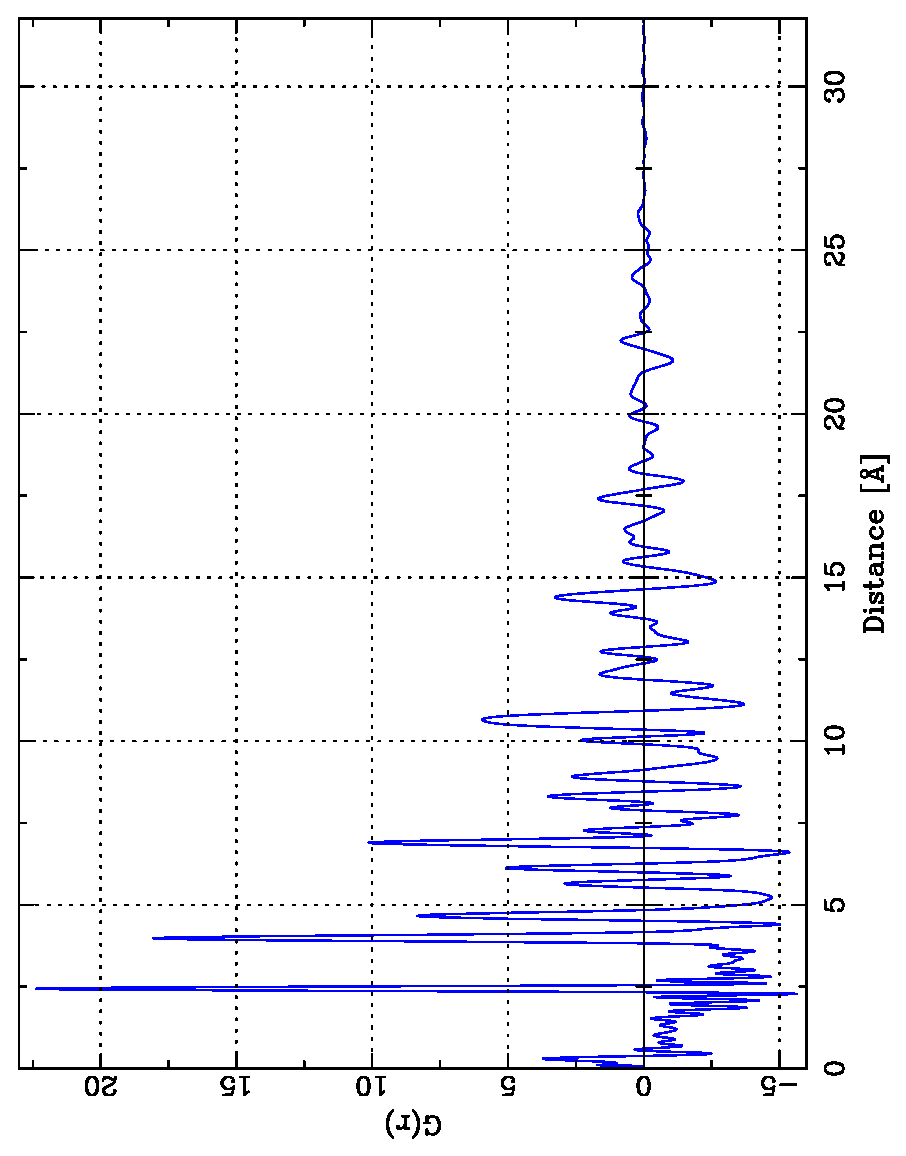
\includegraphics[angle=270,scale=0.45]{znse_grexp.eps}
   \caption{Experimental PDF for ZnSe nanoparticles}
   \label{fexa-znse-grexp}
\end{figure}

The experimental PDF suggests nanoparticles with diameter around 3 to 4 nm.
As bulk ZnSe crystallizes in the Zincblende structure, this provides for
a good starting model. Further modifications include an ellipsoidal shape
rather than a spherical shape and the inclusion of stacking faults that
allow for an alternation of locally cubic and hexagonal sequences. 
The first interatomic distances are observed at 2.44\AA{} and at
3.98\AA{} only. These two distances impose a locally tetrahedral environment,
and the stacking faults have to preserve this environment. TEM images
indicated that lattice fringes across the particles appeared undisturbed.
This is consistent with a model in which one of the symmetrically
equivalent cubic [111] directions is along the long axis of the ellipsoids.
Stacking faults will shift the layers normal to this direction and 
apparently no stacking faults are present along any of the other [111]
directions. 

As the nanoparticles are small, an individual simulated particle that 
contains stacking faults will not be a good representation of all 
possible configurations. See \cite{nedpro} for a full discussion. In the
refinement we will thus have to calculate individual nanoparticles 
several times for each set of parameters and average the corresponding 
calculated PDFs.

The main refinement macro consists of the following steps, which are shortly
outline before we go into the full details:
\begin{MacVerbatim}
diffev                        ! Switch to diffev section
#
  @cleanup.mac                ! Remove old files
#
  REF_NINDIV = 20             ! Define number of individual repetitions
  @get_model.mac              ! Define the refinement model to use
  @diffev_setup.mac           ! Define refinement details
#
  init silent                 ! initialize all parameters, silently no files are written
#                             ! The command can be omitted 
#
  do i[0]=1, 200              ! Number of refinement cycles 
    echo "Loop GENERATION %4d %4d", i[0], REF_GENERATION
    !                         ! Run discus section with macro dis.diffev.mac, no repetitions
    run_mpi discus, dis.diffev.mac, repeat:REF_NINDIV, compute:serial, logfile:LOGFILES/d
    compare silent            ! Compare R-values to previous generation
  enddo
exit                          ! Back to suite
exit                          ! Finish the suite as well
\end{MacVerbatim}
With the first line the \Suite is  instructed to switch to the \Diffev section. 
The {\tt cleanup.mac} macro contains line to remove all files from a previous
refinement run. The commands work on all operating systems and do not ask to
confirm the removal of the files. Next the line REF\_NINDIV  defines the number 
of individual repetitions that need to be performed for each parameter set i.e. 
for each member of the population.

If you look at the remainder of the main macro, you'll notice that 
the vairable REF\_NINDIV 
corresponds to the parameter for the optional {\tt repeat:} on 
the {\tt run\_mpi} line.
You can run the individual repetitions either serially in {\tt dis.diffev.mac}
with {\tt compute:serial} or
run parallel versions of this macro. 
These models are explained 
further down after this quick overview. 

For this example, the user can
specify four different nanoparticle types:
\begin{itemize}
  \item a spherical particle with no stacking faults
  \item a spherical particle with stacking faults
  \item an ellipsoidal particle with no stacking faults
  \item an ellipsoidal particle with stacking faults
\end{itemize}
Macro {\tt get\_model.mac} reads the users choice. If the user had chosen 
a particle with no stacking faults, there will be no need to average
several individual particles. Accordingly, the choice in the main
refinement macro is
overwritten by setting the value of {\tt REF\_NINDIV} to one.
Next, macro {\tt diffev\_setup.mac} does all the detailed setup for the 
refinement. Once the setup is done, {\tt init silent} initializes the first
generation. As of version 5.16 this command can actually be omitted, as 
\Diffev recognizes the state it is in and will perform an initialization
if needed.

In the following loop over a fixed number of refinement cycles 
\Diffev uses the \Discus section to simulate the nanoparticles and to calculate
the agreement between the experimental and calculated PDFs. The {\tt compare}
command instructs \Diffev to compare the current generation to it parents and
to create a next generation of trial parameters.  
The final two lines finish the \Diffev section and the \Suite program itself.

On a Unix type operating system the \Suite program will be started with a line like:

\begin{MacVerbatim}
mpiexec -np 250 discus_suite -macro refine.mac
\end{MacVerbatim}
Alternatively you can usually use {\tt mpirun} and most MPI environments 
will take either {\tt np} ( the proper form ) or {\tt n} to specify the 
number of parallel processes to be started. 

With Windows start a first \Suite window and at the command prompt type:

\begin{MacVerbatim}
parallel refine.mac
\end{MacVerbatim}

An optional parameter allows control over the number of parallel processes as 
well:
\begin{MacVerbatim}
parallel 250, refine.mac
\end{MacVerbatim}

The number of parallel processes that you want to start depends on the 
hardware that is available. On a single PC, do not choose more processes than
the number of cores available. The additional administrative burden will 
actually slow down the over all performance. On a high performance compute 
facility consult the local manual. Usually you will will submit a job into 
a queue. On a modern system you will have a total of several hundred 
processors that are available.

From the model of an ellipsoidal nanoparticle with stacking faults we can
derive 7 structural parameters. Although bulk ZnSe crystallizes in the
cubic Zincblende structure, we will choose to describe the nanoparticle 
based on the hexagonal Wurtzite structure. The cubic lattice parameters can
be transferred into the hexagonal metric via the matrix:
\begin{equation}
  ( \vec{a}_h, \vec{b}_h,\vec{c}_h ) = \left ( \vec{a}_c, \vec{b}_c, \vec{c}_c  \right )
   \left ( \begin{array}{rrr} 1/2 & 0   &1 \\ -1/2 &1/2 &1 \\ 0 &-1/2 &1 \end{array} \right )
\end{equation}

As the Wurtzite structure consists of two alternating layers, while the 
Zincblende structure consists of three layers, the Wurtzite lattice parameters
are actually better obtained by:

\begin{equation}
  ( \vec{a}_h, \vec{b}_h,\vec{c}_h ) = \left ( \vec{a}_c, \vec{b}_c, \vec{c}_c  \right )
   \left ( \begin{array}{rrr} 1/2 & 0   &1/3 \\ -1/2 &1/2 &1/3 \\ 0 &-1/2 &1/3 \end{array} \right )
\end{equation}

This transformation yields hexagonal lattice parameters a=4.008\AA\ c=6.5444\AA. One can 
expect slightly smaller values for the current nanoparticles, as the measurement 
was carried out at 30K. The second neighbor distance at 3.98 is a good estimate 
for the hexagonal a lattice parameter. In an ideal Wurtzite structure both atom
types are located at Wyckoff position 2a 3/3, 1/3, z with z=0 and z=3/8 and we 
will use this value as starting value for the refinement. As Zn (30) and Se (34) 
are very close to each other in the table of elements, and the data were collected
with X-rays, it is not important which element is placed at z=0. Furthermore, as
both sites are symmetrically equivalent, it is a good approximation to use just 
one common atomic displacement parameter for both elements. The experimental PDF
yields significant distances up to approximately 30\AA, and we will use this as
initial estimate for the nanoparticle diameter.

This gives us seven structural parameters:

\begin{itemize}
 \item lattice parameter a 
 \item lattice parameter c 
 \item z-position of Zn
 \item a common isotropic displacement parameter
 \item stacking fault parameter
 \item diameter in the hexagonal a-b plane
 \item diameter along the hexagonal c-axis
\end{itemize}

Beyond this we have parameters for the PDF:

\begin{itemize}
 \item number density
 \item the linear correlation term
 \item the quadratic correlation term
 \item the instrumental dampening term
 \item the instrumental broadening term
 \item the value of Q$_{max}$
 \item the scale factor
\end{itemize}

The instrumental terms and Q$_{max}$ are of course fixed during the refinement.
For this refinement the quadratic correlation term is also fixed at zero, and 
the linear correlation term is refined. We will calculate the PDF from an 
actual simulation of individual nanoparticles that will contain randomly
placed stacking faults. As a consequence, the $-4 \pi \rho_0 r$ line needs to
be corrected for the finite size and shape of the nanoparticle. Currently 
\Discus does not contain any analytical corrections other than that for a
spherical shape. Instead the parameters for an empirical shape function will be 
refined together with the structural model. As this empirical shape function
is completely correlated to the number density we will fix the number density at 
zero and refine the scale factor only.

In total this gives nine parameters to refine. For this number of parameters a 
population size of 90 to 140 members is a good compromise. 

With these initial considerations we are ready for a detailed look at the 
refinement macros. The first macro to consider in detail is 
{\tt diffev\_setup.mac}. The essential lines in the macro are:
\begin{MacVerbatim}
 1: pop_gen[1] =   0
 2: pop_n[1]   =  90
 3: pop_c[1]   =  90
 4: newpara    P_lata, 3.9000,  4.020,  3.900, 4.020
 5: diff_cr[1] = 0.9
 6: diff_f[1]  = 0.81
 7: refine     P_lata
 8: donor      random
 9: selection  best,all
10: trialfile  silent
11: restrial   silent
12: lastfile   DIFFEV/Current
13: logfile    DIFFEV/Parameter
14: summary    DIFFEV/Summary
15: backup TEMP/calc, FINAL/final
\end{MacVerbatim}

The first line sets the generation number to zero. Although this is the default
value at program start, this command is necessary to ensure that \Discus will 
properly start a new refinement. The next two lines set the population and 
children size to 90, ten times the number of parameters to be refined. In the
authors experience it is best to keep the number of parents (= the population
size) and the number of children created in each generation at equal values.

Next we define a (first) new parameter, called {\tt P\_lata}. You are free to 
choose any parameter name as long as it conforms to the variable name restrictions
within the \suite, and consists of 1 to 16 characters. As of version 5.16 this
parameter name is placed into the list of user defined variables and its value 
is passed down to the slave process. Thus, in this example, we will use the
variable {\tt P\_lata} whenever we need to reference the a lattice parameter 
within \discus. The first two numerical parameters are fixed lower and upper
limits for the parameter value. This bracket the expected value of 3.98\AA.
As this window is fairly small already, the starting window is set to identical
values as well. \Discus will assume that this parameter is a real valued 
parameter rather than an integer valued one. 

Further lines have to added for each of the parameters that we wish to refine.
You will find these in the actual macro.

Lines 5 and six set the behavior of the cross-over and the scale factor 
parameters for the differential evolutionary algorithm. In contrast to many
other numerical tasks \cite{prstla2005}, the exact values of the cross-over
probability and the scale factor do not seem to be very relevant for the 
refinement of diffraction data. Keep these parameters as set.

Line 7 specifies that we wish to refine parameter P\_lata. As of version 5.16
this is implied already in the {\tt newpara} command, if the lower and upper 
boundaries differ. The command can actually be omitted.

The \Diffev section offers two choices to determine the donor for each parent.
You can take the donor as the current best member in hope that all new children
will be close to this member and thus hopefully will yield a low R-value. The
alternative choice is to take a randomly chosen member as donor and to add the
difference vector to this member. This latter strategy seems to work better and
is chosen in this example.

For the selection of the members that will produce the following generation,
line 9, two choices are available. The original algorithm makes a choice between
a parent and its child. The better of these two survives to act as parent for the
following generation, even if both the parent and the child have a rather high
R-value compared to the total population. It is a bit more efficient to pool 
all parents and all children into a common group and to select the better half 
of this group as parents for the next generation, as is done in this example in
line 9.

Lines 10 to 14 define the files into which \Diffev will write a log of the 
refinement. As the \Suite can pass the trial parameters directly to the slave 
process and receive back the R-value the need for the trial and result files
has become obsolete. By setting these to a value {\tt silent} their use is 
switched off. The other three lines define the full log for the currently
finished generation, the full log for the complete refinement and the short
summary file for the full refinement. If, as in this example, the files are 
placed into a folder, \Diffev will not check if this folder does exist. You
need to create the folder prior to the refinement. 

In the last line the backup option is defined. \Diffev will expect that the 
slave processes write a diffraction pattern/PDF into the folder {\tt TEMP}
with filenames {\tt calc.0001}, where the four digit number corresponds to the
child number. The currently best files are archived into the folder 
{\tt FINAL} as files {\tt final.0001} etc. This archiving is helpful if you
want to monitor the progress of a lengthy refinement.

The next step in the main macro is the command {\tt init silent}. This command
instructs \Diffev to assign initial values to all parameters. The values are
randomly chosen in the start interval that is defined by the last two 
parameters on the {\tt newpara} command. The {\tt silent} parameter indicates
the no trialfiles are to be written. Instead the \Suite will pass the parameters 
internally to the slave processes. As of version 5.6 this command is not needed.
The \Diffev section will initialize all parameters in generation zero even 
without this command.

This gets us back to the main refinement macro. It performs a loop over 200
or so refinement cycles. \Diffev does allow the user to stop a refinement
upon a variety of convergence criteria. As population based refinements tend
to be stagnant for a while, and since high performance centers usually 
allot a fixed time per run, it is best to choose a fixed number of cycles.
The main workload in each generation is distributed via the command

\begin{MacVerbatim}
    run_mpi discus, dis.diffev.mac, repeat:REF_NINDIV, compute:serial, logfile:LOGFILES/d
\end{MacVerbatim}

This line instructs \diffev to switch to the \Discus section and to execute 
(in parallel) the 
macro {\tt dis.diffev.mac}. The third parameter tells the \Diffev section
how often an individual calculation is to be repeated on the \Diffev side.
With {\tt compute:serial} we tell \Diffev and the \Discus slaves that the
individual repetitions shall be calculated serially within the macro
{\tt dis.diffev.mac}.

The last parameter is the base of logfiles that will receive all output from 
\Discus. The base is augmented by a four digit number for each member of the
population. In the example above files {\tt LOGFILES/d.0001} etc would be written
into the folder {\tt LOGFILES} whose existence you need to ensure prior to the
refinement. Once you are happy with the \Discus macros the parameter can be
omitted or be replaced by {\tt none} or {\tt /dev/null}. In this case the output is
discarded.

If the repetitions are performed on the \Diffev side, the number of tasks that
need to be distributed and can be calculated in parallel is the 
population size times the number of individual repetitions. Once this is 
finished the individual results ( powder diffraction pattern or PDFs) that 
belong to a given member need to be collected, averaged and the agreement 
to the experimental data be calculated. The combination of commands to do 
so would for example be:

\begin{MacVerbatim}
    nindiv   =  50
    pop_c[1] = 100
    run_mpi discus, dis.diffev.mac, repeat:REF_NINDIV, compute:parallel, logfile:LOGFILES/d
    run_mpi discus, kup.diffev.mac, repeat:REF_NINDIV, compute:serial, logfile:LOGFILES/d
\end{MacVerbatim}
Here we use {\tt compute:parallel} to tell \Diffev to run 
the \Discus macro {\tt dis.diffev.mac} 
{\tt pop\_c[0]*nindiv} times. The \Discus macro should be written 
such that it performs exactly one calculation for a given member and 
individual repetition. The second parallel command {\tt run\_mpi} 
instructs \Kuplot to collect the nindiv results for a given member
and to return the agreement factor (R-value) to the \Diffev section.
The maximum number of tasks that can run in parallel is the population
size, her in this example 100. \Kuplot needs to know the number of individual
repetitions, this is done by specifying the {\tt repeat:REF\_NINDIV}
parameter as well. Since \Kuplot has to average all these individual
calculated PDF data, it will work serially on all the individual
repetitions thus the need for {\tt compute:serial}. 

The advantage
of this computational model is that we can run a large number of tasks in parallel with
the first {\tt run\_mpi} command. The disadvantage is the need to store, 
collect and average the individual diffraction pattern/PDFs on a central 
disk to which all the parallel tasks have to have access to.

The alternative model runs only the members of the population in a parallel
fashion. The individual repetitions are performed one after the other on the
one CPU that is calculating a given member. The two {\tt run\_mpi} lines above 
reduce to the one line stated originally: 
\begin{MacVerbatim}
    run_mpi discus, dis.diffev.mac, repeat:REF_NINDIV, compute:serial, logfile:LOGFILES/d
\end{MacVerbatim}

As of version 5.17.0 the number of individual repetitions will still be 
handed down to {\tt dis.diffev.mac}.  The macro has to 
branch into \Kuplot in order to average individual calculations. The 
disadvantage of this model is the much smaller number of tasks that can be run 
in parallel. The number of parallel tasks should only be a fraction of the 
population size. This will ensure that each node or CPU will perform several 
calculations and all nodes will -hopefully- finish at the approximately same
time. The advantage of this model is the considerably reduced data I/O. All
individual results do not have to be written onto the hard disk at all. Instead
\Discus can write these directly into the \Kuplot memory. 

Whether to perform individual repetitions on the \Diffev side or on the
\Discus side depends on the computational hardware that is available. 
On a local PC you typically have one node with likely some four to eight CPUs,
one common storage disk, and possibly a smaller yet faster (temporary) 
solid state disk. 
At a HPC you usually have many nodes that work in parallel each with several
CPUs. While there is one common storage disk, each nodes will have its own 
(temporary) and fast storage as well. The central storage is optimized towards
huge files that are written every once in a while. Small temporary file input
 and output is to be avoided onto this central storage, as it put a huge burden 
on the communication between the nodes. 

Unfortunately the message passing interface (MPI) that \Diffev uses to perform
the refinement in parallel does not allow an easy assignment of individual tasks
onto a specific node, nor does it have an easy way to let the central master 
program know on which node a given task was calculated.  This limitation 
favors the model where individual repetitions are performed serially by the
\Discus macro. Future hybrid releases of the \Suite may improve at this point.
As of version 5.17.0 \Diffev will place all individual repetitions of a given
member onto the same node, eliminating the MPI disadvantages. Thus a compute
model with parallel distribution of the individual repetitions is recommended.

The essential lines in the macro {\tt dis.diffev.mac} are:
\begin{MacVerbatim}
 1: set error,exit
 2: variable integer, indiv
 3: @get_model.mac
 4: @global.mac
 5: #
 6: do indiv = 1, REF_NINDIV
 7:   @discus.znse.mac
 8: enddo
 9: branch   kuplot    !Switch to KUPLOT
10:    @kup.diffev.mac
11: exit
\end{MacVerbatim}

This is a fairly generic macro that needs little change from one refinement to
another. Line 1 sets a strict termination, if any error should occur in subsequent
macros. This prevents a refinement from running on and on if something went wrong
in the refinement. Line 2 defines a local variable for the loop in lines 6 to 8.
In this loop we go over all the individual repetitions for the current parameter 
set, i.e. for the current member of the population. 

Line 3 might have to be adapted to a different refinement. In this examples it
determines the model that is to be used. The macro is identical to the one used 
in the main refinement macro. 

Line 4 runs a macro {\tt global.mac} that is used to set several filenames. By
collecting all these file name definitions in one central macro it becomes less
tedious to adapt to different substances, data files etc.

Lines 6 to 8 run a loop over all the individual repetitions that are required if
a simulation involves randomly placed defects. Often an individual object created
in a simulation is not large enough to hold a good representation of the defect
distribution. In these cases one has to build several structures according to 
the same rules. In a second step all the diffraction pattern or PDFs need then 
to be averaged. If the model does not involve statistically distributed defects,
all that you have to do is omit the loop or more simply set the number of 
iterations {\tt nindiv} to one. The macro {\tt get\_model.mac} does exactly this, if
the user decides on a model of a perfect crystal without stacking faults. For
this model, all nanoparticles are identical and it is sufficient to create just 
a single one.

In line 7 we run the main work horse {\tt discus.znse.mac}. This macro has of 
course to be adapted in detail for a different type of refinement. We will go
through this macro in the following section.

In lines 9 and 10 we branch from the \Discus section to the \Kuplot section
in order to average the calculated PDFs and to calculate the agreement factor
to the observed data.

Finally, in line 11 the \Discus section is terminated which will return the 
control to the master process. If there are still tasks to be distributed the 
current slave process will receive a new task and repeat the steps discussed 
for this macro.

The style adopted in this macro {\tt dis.diffev.mac} corresponds to the first
style defined in section \ref{diff-parallel}. The individual repetitions are
computed serially by one slave process. Accordingly we will use internal 
storage of the individual output data and calculate the R-value in the branch
to \Kuplot in lines 9 and 10. For this style a suitable {\tt global.mac} would be:
\begin{MacVerbatim}
 1: variable character, TMPDIR    ! temporary DISCUS files   'internal'     or '.'
 2: variable character, INDIDIR   ! temporary PDF directory  'kuplot'       or '.'
 3: variable character, DATADIR   ! input data directory     '/tmp/mpkr04/' or '.'
 4: variable character, DATAFILE  ! Input Data File  
 5: variable character, SUBSTANCE ! Substance name
 6: DATADIR   = "%c",'/tmp/zzzzzz'
 7: DATAFILE  = "%c",'PD32ZS56.DAT'
 8: INDIDIR   = "%c",'kuplot'
 9: TMPDIR    = "%c",'internal'
10: SUBSTANCE = "%c",'znse_wurtzite'
\end{MacVerbatim}

The \Kuplot macro {\tt kup.diffev.mac} will copy the experimental data 
{\tt DATAFILE} to a temporary
location at {\tt DATADIR}. This serves to reduce network traffic during the refinement,
see the macro {\tt kup.diffev.mac} further down. Make sure that the directory
{\tt /tmp/zzzzz} exists and that you have write privileges. At a local PC or local
small server you could use the line 
\begin{MacVerbatim}
 6: DATADIR   = "%c",'.'
\end{MacVerbatim}
instead. This would place the copies to a local directory in your current 
working directory.   {\tt TMPDIR} is a directory to 
temporary \Discus structure files. Except for debugging purposes you can keep this
as {\tt internal}, which will place these files into the internal memory structure
of \Discus without unnecessary disk input/output. As this compute style will calculate
all individual repetitions serially in one call to macro {\tt dis.diffev.mac}, we
do not have to write these files to a disk. See the macro {\tt pdf.mac} further
down to see how the string {\tt INDIDIR} 
is placed at the beginning of these temporary  output files.  As the string has the 
value {\tt kuplot} \Discus is instructed not to write the files onto disk but to copy 
them directly into the  \Kuplot memory.

For the second style in \ref{diff-parallel} we leave it to \Diffev to distribute
the calculation of individual repetitions to separate slave processes. in this case
macro {\tt dis.diffev.mac} should read:
\begin{MacVerbatim}
 1: set error,exit
 2: variable integer, indiv
 3: @get_model.mac
 4: @global.mac
 5: #
 6: indiv = REF_INDIV
 7:   @discus.znse.mac
 8: enddo
 9: exit
\end{MacVerbatim}
Note that in line 6 we assign the value of {\tt REF\_INDIV} to our local variable
{\tt indiv}. {\tt REF\_INDIV} is a global variable set by \Diffev along with 
{\tt REF\_KID} to the individual repetition number. This assignment allows us to
use all further macros without change. The branch to \Kuplot is omitted, as the
main refinement macro {\tt refine.mac} will now include a separate {\tt run\_mpi}
statement to run the \Kuplot calculations. 

The only change needed for {\tt global.mac} is:
\begin{MacVerbatim}
 9: INDIDIR   = "%c",'/tmp/zzzzzz'
\end{MacVerbatim}
As the \Suite (starting with version 5.17.0) places all individual repetitions
onto the same node of your cluster, these temporary output files for one 
member of the population will all be at the same local directory {\tt /tmp/zzzzzz}
and thus be accessible to the second {\tt run\_mpi} step in which 
\Kuplot is used and the Rvalue is calculated. 


The main simulation macro {\tt discus.znse.mac} consists of the essential lines:
\begin{MacVerbatim}
 1: variable real, P_qmax
 2: P_qmax      = 30.00
 3: #
 4: read
 5:    free P_lata, P_lata, P_latc, 90.00, 90.00, 120.00, P63mc
 6: insert Zn, 1./3., 2./3., P_z_zn, P_biso
 7: insert Se, 1./3., 2./3., 0.0000, P_biso
 8: #
 9: if(model.eq.PERFECT_SPHERE .or. model.eq.PERFECT_ELLIPSOID) then
 0:    P_stack  = 1.00
11: endif
12: #
13: if(model.eq.PERFECT_SPHERE .or. model.eq.STACKED_SPHERE) then
14:    P_cc_dia     = P_ab_dia  !ref_para[ 06]    ! Spherical model
15: endif
16: #
17: save
18:   outfile "%c/STRU/%c.%4D.%4D.cell", TMPDIR,SUBSTANCE,REF_KID,indiv
19:   run
20: exit
21: @makelayers.mac
22: #
23: @shape.ellipsoid.mac
24: @pdf.mac
\end{MacVerbatim}

In lines 1 and 2 we begin by defining the Q$_{max}$ value that was used in the 
actual experiment to derive the experimental PDF. It would be sufficient to
write this number explicitly in the pdf macro that is executed in line 24.
I prefer to write this value at this point, as this makes the pdf macro a
completely generic macro that does not have to be changed at all for the
refinement of another nanoparticle pdf. If the number id encoded in the actual 
macro it increases the chance to forget to change this number.

Lines 4 to 7 are used to create the asymmetric unit for the Wurtzite type ZnSe 
structure. Check the \Discus manual for full details of these commands. The 
important point to mention here is that all variables in this macro that start
with {\tt P\_} are parameters that are to be refined. The parameters were
defined in the macro {\tt diffev\_setup.mac}. OK, the exception to this
rule is {\tt P\_qmax} the fixed value for Q$_max$. \Diffev does not impose any
rule on the parameter names that you choose, as long as they are regular variables
that are valid in any section of the \Suite and whose name consist of up to 16
characters.  The {\tt free} command creates general coordinates system, here a
hexagonal coordinates system. The last parameter defines the space group intended.
The Wurtzite structure consists of two atoms in space group P6$_3$mc. Both atoms
are at the position 1/3, 2/3, z. We can fix the z position of one of the two 
atoms at an arbitrary value. Here Se is fixed to z=0, while the z position of
Zn is to be refined. Its z value will be close to 3/8, the value in the 
idealized Wurtzite structure.

In lines 9 to 11 and 13 to 15, respectively, restrictions that are imposed by
the model are applied to the parameters. If the user intends to model a 
perfect nanoparticle without stacking faults, the parameter is set to one, 
which will result in a perfect Zincblende structure type. Similarly, if a 
spherical nanoparticle is intended, the diameter {\tt P\_cc\_dia} along the 
hexagonal c-axis is fixed to a value identical to the diameter in the a-b plane.
These local changes to the parameter values do not affect the value of the 
parameters within the scope of the master process. If the master process tries to
refine these parameters, no sensible results will be obtained for the parameters
if the local restrictions are applied.

As lines 4 to 7 have created the asymmetric unit only, this asymmetric unit is
saved in lines 17 to 20. This will enable later parts of the macro to read the
modified asymmetric unit and to expand it to a full crystal. The value of 
the character variables {\tt TMPDIR} and {\tt SUBSTANCE} is set within macro
{\tt global.mac}. For this example the variable {\tt TMPDIR} is set to a value
{\tt internal}. \Discus saves any file that starts with the string "internal" 
within an internal memory structure rather than to write the file to the hard
disk. As the current asymmetric unit is a temporary file there is no need to 
write the file. During the development of a refinement it might be a good idea
to write the file to the hard disk in order to ease debugging processes. As 
the refinement shall eventually run in parallel, it is mandatory that all files
that are written to the hard disk have a unique file name. For that reason the 
current member number and individual repetition number are added to the file
name.

In this refinement we intend to stack layers of the hexagonal Wurtzite structure
type in order to create a disordered sequence of layers. As the interatomic
distances are to be refined, the layer structures will vary as function of the
refinement parameters. Macro {\tt makelayers.mac} in line 22 creates  these new
layers that are needed for the Wurtzite/Zincblende stacking sequence.

The macro {\tt shape.ellipsoid.mac} does the actual stacking process and includes
commands to shape the particle into an ellipsoidal shape.

Finally in line 24 macro {\tt pdf.mac} is used to calculate the PDF for this 
current simulation.

Once the PDF is calculated the macro {\tt dis.diffev.mac} continues with the average
process and evaluation of the R-value through the \Kuplot section.

The discussion will continue with a detailed look at the nanoparticle build up.
First lets look at {\tt makelayers.mac}

The atom positions in the (idealized) Wurtzite type structure are located at:
\begin{MacVerbatim}
   Zn  2/3,  1/3, -1/8     A
   Se  1/3,  2/3,  0       b
   Zn  1/3,  2/3,  3/8     B
   Se  2/3,  1/3,  1/2     a
   Zn  2/3,  1/3,  7/8     A
   Se  1/3,  2/3,  1       b
   ...
\end{MacVerbatim}

The letters ABAB denote the layer sequence of the Zn atoms, the small letters
abab the corresponding sequence of the Se atoms. The whole structure can be 
described as a sequence of (Ab)(Ba)(Ab)(Ba) double layers. Within a (Ab)
double layer the vector from Zn to Se is [-1/3, +1/3, 1/8], while the
corresponding vector in the (Ba) double layer is [+1/3, -1/3, 1/8]. The
Wurtzite structure can thus be described as a ABAB Sequence of two different 
layer types (Ab) and (Ba). The (Ba) double layer can be created by rotating 
the (Ab) double layer by 180° around the c-axis. With this notation, the
perfect Zincblende structure type results if either pure (Ab) double layers 
or pure (Ba) double layers are stacked in a sequence of ABCABC...
Mixed layer types result if the sequence of (Ab) and (Ba) layers is modified.
\begin{MacVerbatim}
 1: # makelayers.mac
 2: #
 3: variable integer,width
 4: variable real, thick
 5: width = int(2.5 * P_ab_dia/P_lata )
 6: #
 7: read
 8:    cell "%c/STRU/%c.%4D.%4D.cell",TMPDIR,SUBSTANCE,REF_KID,indiv,width,width,2
 9: thick = blen(0.0, 0.0, 0.5-P_z_zn) + 0.1
10: #
11: surface
12:    boundary hkl, 0, 0, 1,   0.5,inside
13:    boundary hkl, 0, 0,-1, thick,inside
14: exit
15: purge
16: #
17: save
18:    outf "%c/STRU/%c.%4D.%4D.layer",TMPDIR,SUBSTANCE,REF_KID,indiv
19:    write all
20:    run
21: exit
22: #
23: symm
24:    angle 180.0
25:    type  proper
26:    mode  repl
27:    sel   all
28:    incl  all
29:    orig  0.333333, 0.666667, 0.00
30:    uvw   0,0,1
31:    trans 0.00, 0.00, 0.00
32:    run
33: exit
34: #
35: save
36:    outf "%c/STRU/%c.%4D.%4D.rotated",TMPDIR,SUBSTANCE,REF_KID,indiv
37:    run
38: exit
\end{MacVerbatim}

Macro {\tt makelayers.mac} builds these two layer types. Two strategies 
could be used to perform this task. You could either build a large template
of (Ab) and (Ba) and then modify the atom coordinates of Zn relative to Se
to adjust the refined lattice parameters and the z-position of Zn. 
Alternatively the whole layer can be recreated from the modified asymmetric 
unit. Here the latter strategy es employed. The allows for more flexibility
to build a layer of arbitrary size to ensure that the final nanoparticle 
will fit inside the layer.

In line 5 variable width is calculated to be large enough to include the
final nanoparticle with diameter {\tt P\_ab\_dia} in the hexagonal a-b plane.
The factor 2.5 is a bit generous to ensure that at no corner of the hexagonal 
space we will cut off atoms inside the intended diameter. In lines 7 and 8
the asymmetric template generated in {\tt discus.znse.mac} is read and 
expanded to a width by width by 2 unit cells.  The {\tt surface} menu in
lines 11 to 14 cuts off all atoms above the (0,0,1) surface located at
a distance of 0.5 \AA\ above the origin and all atoms below the (0,0,-1)
surface located ad a distance of {\tt thick} below the origin. The value 
of {\tt thick} is calculated from the refinement parameter {\tt P\_z\_zn}
as idealized 1/2 - 3/8 = 1/8 along the c-axis. This places the (0,0,-1) plane
just below the position of the Zn atoms at 2/3,  1/3, -1/8. All other atoms
are no longer needed and removed by the  {\tt purge} prior to saving the 
layer in lines 17 to 21. Next the layer is rotated by 180$^\circ$ around the
c-axis. Note that the rotation axis is placed at the Se position 1/3, 2/3, 0 to
ensure correct stacking later on.

After these preparations we are now ready to build the actual nanoparticle
inside our next macro {\tt shape\_ellipsoid.mac}.
\begin{MacVerbatim}
 1: read
 2:    cell "%c/STRU/%c.%4D.%4D.cell",TMPDIR,SUBSTANCE,REF_KID,indiv
 3: #
 4: @stack.mac
 5: #
 6: surface
 7:    boundary ellipsoid, P_ab_dia, P_ab_dia, P_cc_dia, centx:0.0,centy:0.0,centz:P_cc_dia*0.5/P_latc
 8: exit
 9: purge
\end{MacVerbatim}

The macro is short and all of its lines could easily have been placed inside
the main macro {\tt discus.znse.mac} without making the main macro too long
and too difficult to follow. Subdividing the macros does make it easier to
modify the main macro by just changing one line. 

The macro begins by reading the template again and expanding it to just one 
unit cell. This is done to ensure that the stacking sequence in {\tt stack.mac}
works on the correct metric, even if the main macro might later on be changed to
work on further structures. Macro {\tt stack.mac} does build the actual 
particle. Once it is done the {\tt surface} menu is used to shape the 
crystal into a triaxial ellipsoid with diameters P\_ab\_dia, P\_ab\_dia,
and P\_cc\_dia. Even though we are in hexagonal space, the three half axes
of the ellipsoid are orthogonal to each other. See the \Discus manual 
and on-line help for further details.  The center of the ellipsoid is placed
at half the diameter along the c-axis. The {\tt stack} menu in \Discus
always places the first layer at the origin, thus the need to shift the 
center of the ellipsoid.

The essential lines in {\tt stack.mac} are:

\begin{MacVerbatim}
 1: variable integer,height
 2: height = int(2.*P_cc_dia/lat[3] + 2)
 3: #
 4: stack
 5:    layer "%c/STRU/%c.%4D.%4D.layer"  ,TMPDIR,SUBSTANCE,REF_KID,indiv
 6:    layer "%c/STRU/%c.%4D.%4D.rotated",TMPDIR,SUBSTANCE,REF_KID,indiv
 7:    trans  1,1, -0.3333, 0.3333, 0.5000
 8:    trans  1,2,  0.3333,-0.3333, 0.5000
 9:    trans  2,1, -0.3333, 0.3333, 0.5000
10:    trans  2,2,  0.3333,-0.3333, 0.5000
11: #
12:    number height
13: #
14:    distr  matrix
25:    crow   1,       P_stack, 1.00-P_stack
26:    crow   2,  1.00-P_stack,      P_stack
27: #
18:    aver   0.00, 0.00, 1.00
19:    modu   1.00, 0.00, 0.00,  0.00, 1.00, 0.00
20:    set mod ,on
21:    set trans,fixed
22: #
23:   create
24:   run
25: exit
\end{MacVerbatim}

We start by calculating the height of the stack in numbers of layers,
line 2 and line 12.  The factor "2" in the calculation is due to the fact 
that there are two of the double layers per unit cell in the Wurtzite 
structure type. Two further layers are added to avoid cutting off atoms 
due to rounding errors if the ellipsoid diameter is almost an integer 
multiple of the c lattice parameter. 

Within the {\tt stack} menu (line 4) we first define the two layer types
that comprise the stacking sequence (lines 5,6). The four {\tt trans}
commands define the translation vector from one layer type to the
next layer type. Lines 8 and 9 are the vectors within a perfect Wurtzite
structure type, a perfect Zincblende structure type results with a 
sequence of layer types 1 only (line 7) or layer types 2 only (line 10).  

\Discus offers two different modes to determine the actual stacking sequence.
In this example we use a probability matrix (line 14). The matrix elements
define the probability that a layer type is followed by another layer type.
As we have two layer types, we need the two rows of this matrix (lines 25, 26).
Element (1,1) = P\_stack gives the probability that a layer of type 1 is
followed by a layer of type 1. Likewise element (1,2) = 1 - P\_stack gives the 
probability that a layer of type 1 is followed by a layer of type 2.
In this example, a value of P\_stack close to +1 would result in an (almost)
perfect Zincblende type sequence of layers of type 1, all shifted by the 
translation vector (line 7) [-1/3, 1/3, 1/2]. If the first layer happens 
to be chosen by the program to be type 2 an analogous Zincblende sequence of
layer type 2 would result. A value of just about zero on the other hand,
would result in an (almost) perfect Wurtzite type alternation of layer 
types 1 and 2, separated by vectors (line 8) [1/3, -1/3, 1/2] for type 1 
followed by type 2 and (line 9) [-1/3, 1/3, 1/2] for layer type 2 followed 
by layer type 1.

In order to ease the final shaping of the ellipsoid, lines 18 to 21 define
an average growth direction along vector [0,0,1] (line 18). As soon as the
translation vectors from lines 7 to 10 place the next layer at a location
further away from the c-axis than either of the two modulo vectors on line 19
the layer is shifted back by this modulo vector. As these two vectors [1,0,0]
and [0,1,0] are integer lattice vectors this shift does not have any 
consequences other than to ensure that each layer origin is approximately
at x and y equal to zero. Line 20 turns this modulo behavior on and
line 21 ensures that the average growth direction is taken as the vector 
on line 18. Without this modulo operation a stacking fault parameter of
1 (or close to) would result in a shift of [-1/3, 1/3, 1/2] between any
layer pair. The stack would be an oblique tower. For such an object the 
shaping of an ellipsoid becomes more tedious, as the required horizontal
extend of each layer becomes linked to the vertical height and the stacking
parameter.

Finally we {\tt create} all layer origins (line 23) and build the actual
list of atom coordinates within each layer (line 24). The separation of 
these two steps allows \Discus a tremendous gain in speed when calculating
the diffraction pattern for large crystals. Here, for the ellipsoidally
shaped object both steps have to be done.

Finally macro {\tt pdf.mac} calculates the pair distribution function (PDF)
for the nanoparticles. 
\begin{MacVerbatim}
 1: @setup_pdf.mac
 2: #
 3: pdf
 4: #
 5:     ides all
 6:     jdes all
 7:     isel all
 8:     jsel all
 9: #
10:     set bound,    crystal, exact
11:     set dens,     P_density
12:     set corrlin,  P_corrlinear
13:     set corrquad, P_corrquad
14:     set srat,     P_srat,3.5
15:     set therm,    gauss
16:     set qbroad,   P_qbroad
17:     set qdamp,    P_qdamp
18:     set qmax,     P_qmax
19:     set rad,      xray
20:     set range,    pdf_range+5.0, 0.01
21:     set weig,     P_scale
22:     set finite,   periodic
23:     calc
24:     save pdf,"%c/INDI/indi.%4D.%4D"  ,INDIDIR, REF_KID, indiv
25: exit
\end{MacVerbatim}

In line 1 the variable {\tt pdf\_range} and its value are defined. This 
variable is used in line 20 to define the distance range over which the 
PDF is to be calculated. As the computation time scales with this value
you might want to adapt it to test models over different refinement 
ranges or for differently sized nanoparticles. By placing this information
into a short macro by itself, other parts of the macro suite can use the 
identical macro {\tt setup\_pdf.mac} and there is only one place that needs
modification. After a clean selection of atom pairs for which to calculate
the PDF (lines 5 to 8) all PDF parameters are set (lines 10 to 22). 
The PDF is calculated in line 23 and the data saved in line 24.


At this point macro {\tt discus.znse.mac} returns control to macro
{\tt dis.diffev.mac} which in turn branches off to the \Kuplot
section and performs the macro {\tt kup.diffev.mac}

\begin{MacVerbatim}
 1: variable integer,indiv       ! Local variable for repetition
 2: @global.mac                  ! Directory names 
 3: @get_model.mac               ! Get the refinement model to use
 4: @kup.average.mac             ! Merge all individual calculations REF_NINDIV + 1
 5: load xy, "%c/DATA/%c.%4D", DATADIR, DATAFILE, REF_KID !              REF_NINDIV + 2
 6: spline REF_NINDIV+1, REF_NINDIV +2   ! Ensure identical x-axis-scale REF_NINDIV + 3
 7: @kup.fit.polynomial.mac      ! Correct 4PI RHO line and scale    REF_NINDIV + 7
 8: rval REF_NINDIV+2, REF_NINDIV+7, dat ! calc R-value, is transferred internally
 9: reset                        ! No DATA
10: exit                         ! Back to DISCUS / DIFFEV (depends on use)
\end{MacVerbatim}

In line 1 we define a variable {\tt integer}, which is used inside the macro 
{\tt kup.average.mac} to loop over the individual files. Lines 2 and 3 repeat
the definitions encountered in the main macro {\tt refine.mac}. The next
macro {\tt kup.average.mac} serves to average the individual files created
in the main discus macro {\tt discus.znse.mac}. Next, in line 5, we load the
experimental PDF into \Kuplot. Line 6 could be omitted, if you make sure
that the experimental data and the calculated data are on an identical 
x-scale. As it stands, the {\tt spline} command tells \Kuplot to create a
new data set, with the X-scale taken from the data set indicated by the 
second parameter. The y-scale is calculated as a spline function through 
the y-values of the data set specified by the first parameter. 
As the shape of the nanoparticles might be highly irregular, the 
PDF in {\tt pdf.mac} was calculated with a number density of zero. The 
actual value and the corrections to the $-4 \pi \rho_0 r$ line are applied
in macro {\tt kup.fit.polynomial.mac} (line 7). At this point we are 
ready to calculate the agreement between the experimental and calculated
PDF in line 8. The last parameter signals that the experimental uncertainties
are taken into account for the R-value calculation. A the {\tt reset} in line 
9 tells \Kuplot to remove all loaded data sets. Finally we {\tt exit} the 
\Kuplot macro in line 10.

Note that in lines 6 and eight we do not refer to absolute data set numbers.
Instead the data sets are labeled with reference to the number of individual
repetitions {\tt REF\_NINDIV}. This is necessary, as the number of individual
repetitions may change from refinement to refinement. The current macro 
should work for any number of repetitions. Before we look in detail at 
this numbering scheme, lets look into {\tt kup.average.mac}
\begin{MacVerbatim}
1: if(n[1]==0) then
2:   reset
3:   do indiv=1,REF_NINDIV
4:      load xy,"%c/INDI/indi.%4D.%4D", INDIDIR, REF_KID, indiv
5:   enddo 
6: endif
7: merge all    ! creates new data set number: REF_NINDIV + 1
\end{MacVerbatim}

As explained above, the \Discus macro may either save the calculated data 
sets onto a hard disk, or save them directly into \Kuplot. In the first
case, \Kuplot will at this point be void of data sets i.e. $n[1]=0$, and
the {\tt if} block will be executed. Within the block, the {\tt REF\_NINDIV}
data sets are loaded in the loop. If \Discus did save the calculations
directly into \Kuplot, the {\tt REF\_NINDIV} data sets will already be 
loaded into \Kuplot. In both cases \Kuplot will at this point have loaded
{\tt REF\_NINDIV} data sets. As this number may vary, is is best to refer
to this relative number rather than to specify an absolute value in all 
subsequent \Kuplot macros. Finally, in line 7 these data sets are merged.
As a consequence we will now have {\tt REF\_NINDIV + 1} data sets loaded
into \Kuplot.

Loading the experimental PDF in line 5 of macro {\tt kup.diffev.mac} 
places this experimental PDF into data set {\tt REF\_NINDIV+2}

Macro {\tt kup.fit.polynomial.mac} 
fits a polynomial background to yield an empirical description of the
$-4 \pi \rho_0 r$ line.

\begin{MacVerbatim}
 1: kcal sub,REF_NINDIV+2,REF_NINDIV+3 ! Creates data set REF_NINDIV + 4
 2: skal                      ! Fit needs to know x and y range
 3: fit REF_NINDIV + 4        ! Fit a function to data set REF_NINDIV + 4
 4:   func, poly,6            ! Polynomial of order x**6
 5:   para 1,0, 0.00          ! x^0 is fixed to 0.00
 6:   para 2,1, 1.00          ! x^1 refined, starts at 1.0
 7:   para 3,1, 0.00          ! number, flag, starting_value
 8:   para 4,1, 0.00
 9:   para 5,1, 0.00
10:   para 6,1, 0.00
11:   para 7,1, 0.00          ! x^6 refined, starts at 0.00
12:   wic  dat                ! Use weights inherited from data set
13:   cycle 200               ! 200 cycles should be enough
14:   urf 0.5                 ! control refinement speed ~1/urf
15:   run                     ! Lets do it
16: exit                      ! back to main KUPLOT menu
17: kcal add,REF_NINDIV+3,REF_NINDIV + 5 ! Add polynomial to merged PDF's
18: ksav REF_NINDIV + 7           ! Save this calculated PDF 
19:    outf "TEMP/calc.%4D",REF_KID
20:    run                    ! automatically returns to main menu
\end{MacVerbatim}

In line 1 we subtract the experimental PDF, data set {\tt REF\_NINDIV+3}
from the merged calculated PDFs, data set {\tt REF\_NINDIV + 2}. This
command stores the result in the next available data set 
{\tt REF\_NINDIV + 4}.
Next, we scale the plot (although nothing is plotted to screen) as the 
fit needs to know the x-range over which we want to refine something.
Within the {\tt fit} menu (line) 3 we fit a calculated function to data set 
{\tt REF\_NINDIV + 4}. The function is defined in line 4 as a polynomial
of order 6. This order ensures that quite complex nanoparticle shapes
can be modelled. A (much) higher order would mask deficiencies of the 
nanoparticle model. 
Lines 5 to 11 define starting values for the seven parameters
from $P_1 \times x^0$ to $P_7 \times x^6$. 
The three parameters to the {\tt para} command are: Parameter number, 
refinement flag (0=fixed, 1=refined) and starting value.
Starting values are 0.00 for all parameters except the linear term (line 6). 
The constant term (line 5) is fixed at zero to ensure that the polynomial
goes through the origin at x=0.0, G(r) = 0.0.

The weighting scheme (line 12) uses the uncertainties inherited into the 
difference between experimental PDF and merged calculated PDF. Line 13
defines 200 refinement cycles, sufficient for this linear least squares 
problem. The {\tt urf} parameter defines the speed by which \Kuplot 
changes its refined parameters from cycle to cycle. A large number means slower
convergence as the parameters are changed by smaller amounts.

The {\tt fit} menu creates two further data sets, the calculated function
and the difference between the input data set and the calculated function.
As the input data set is {\tt REF\_NINDIV + 4} (line 3) these new data sets are
{\tt REF\_NINDIV + 5}  and {\tt REF\_NINDIV + 6}. We now add (line 17) 
the calculated polynomial function (data set {\tt REF\_NINDIV + 5}) 
to the input data set. The resulting data set {\tt REF\_NINDIV + 7} 
is the final calculated PDF that will hopefully match the experimental
PDF very well.

Lines 18 to 20 are used to save a copy of the final data set to hard disk.
This save enables the use of the {\tt backup} command in 
macro {\tt diffev\_setup.mac}. This option enables you to have a look 
at the current best calculated PDFs while the refinement is still ongoing.
If you do not need this option, for example while you run a refinement
on a high performance compute center you can omit these lines.

Control is returned to {\tt kup.diffev.mac} which finishes with the
calculation of the R-value (line 8), a reset (line 9) and the exit 
back to \Discus.

\Kuplot calculates the aggreement between the two data sets according
to Eq. \ref{eq-exa-rval}.

\begin{equation}
   wR = \sqrt{\frac{\sum_{i} w_{i} (y_{obs}(i) - y_{calc}(i))^2}
                   {\sum_{i} w_{i} y_{obs}(i)^2}}
  \label{eq-exa-rval}
\end{equation}

Here $y_{obs}$ and $y_{calc}$ are the observed and calculated function
values, in our current example the PDF. The weighting scheme $w_{i}$
assigns a weight to each individual data point. For a diffraction
pattern the weight is commonly $1/\sigma^2$, where $\sigma$ is the
uncertainty of the experimental data point. Currently the commonly
available data treatment software will not provide an uncertainty 
for each data point in the experimental PDF. A unit weight is 
most often used. As the errors in the PDF tend to decrease with 
increasing distance r, a weighting scheme with $\sigma \propto 1/r$
is also used. As the values of the PDF below a distance of 
approximately 1\AA are not reliable, these data points should 
receive a low weight, respectivaly a high uncertainty.

At this point we have gone through all macros that are part of the 
nanoparticle refinement.





\section{Noisy example function}

\begin{figure}
   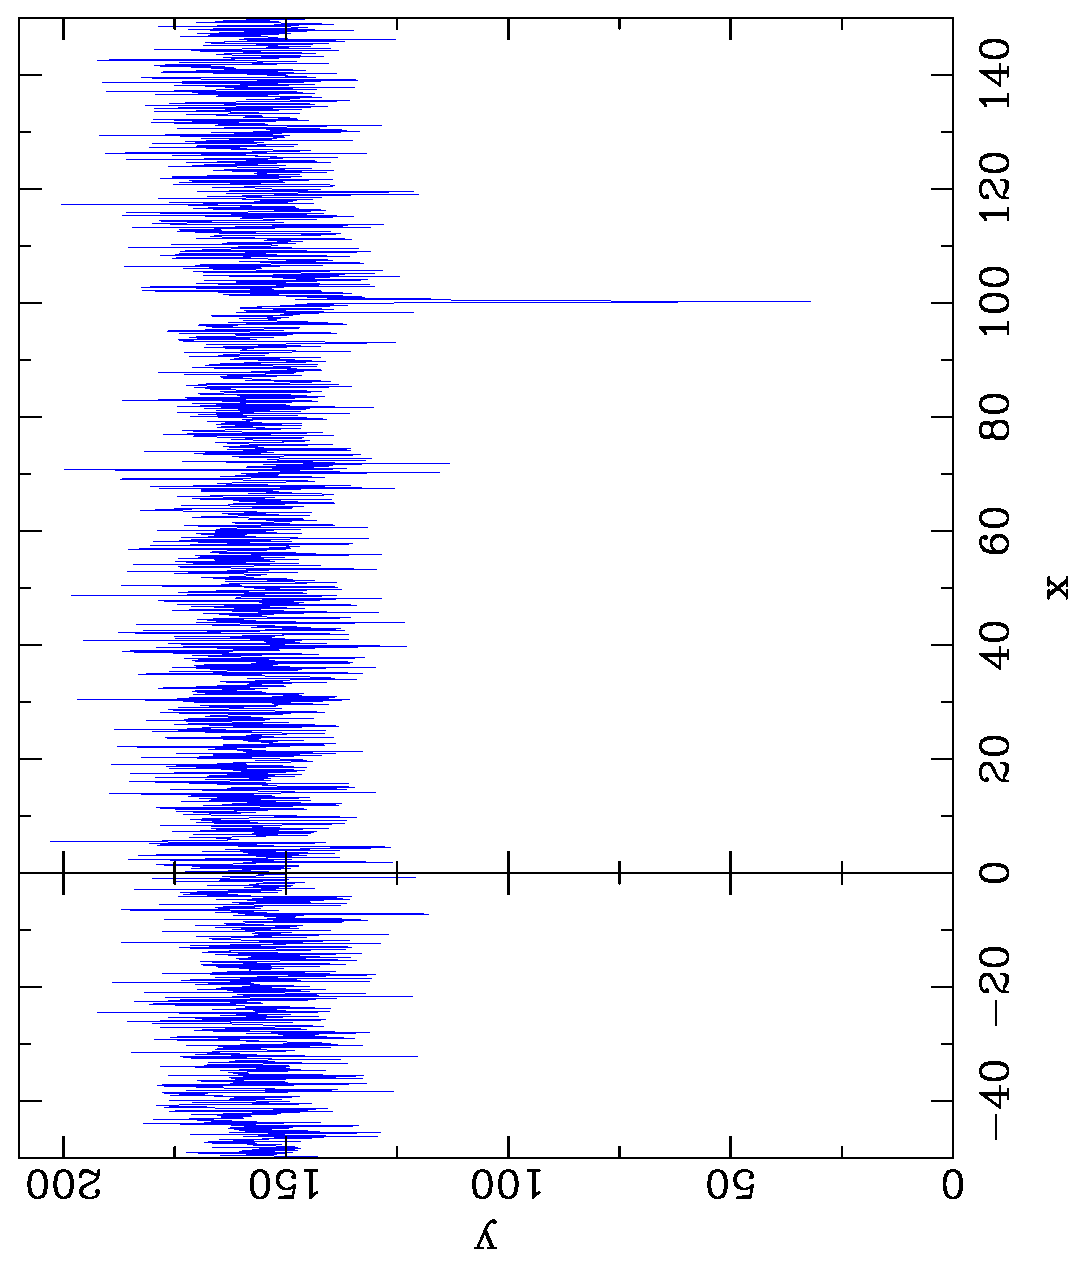
\includegraphics[angle=270,scale=0.45]{example.raw.eps}
   \caption{Example data}
   \label{fexa-arc}
\end{figure}

The function in Fig. \ref{fexa-arc} shall be the data set for the
refinement in this section. The function from which these data were
calculated is:
\begin{equation}
   y ~=~ P_{1} atan \left ( \frac{|x-P_{2}|}{P_{3}}\right)
   \label{eq-exa-arc}
\end{equation}
where atan is the arc tangens or inverse tangens function, and $P_{i}$
are free parameters that determine the behavior of the function. The
function has a minimum y=0 at $x ~=~ P_{2}$. The width of this minimum
depends on $P_{3}$. For small values of $P_{3}$ the minimum is smaller.
Far away from the minimum, the function is almost constant at 
$y ~=~ \pi/2 P_{1}$. The data were generated by adding a Gaussian 
distributed noise to each data point.

\begin{figure}
   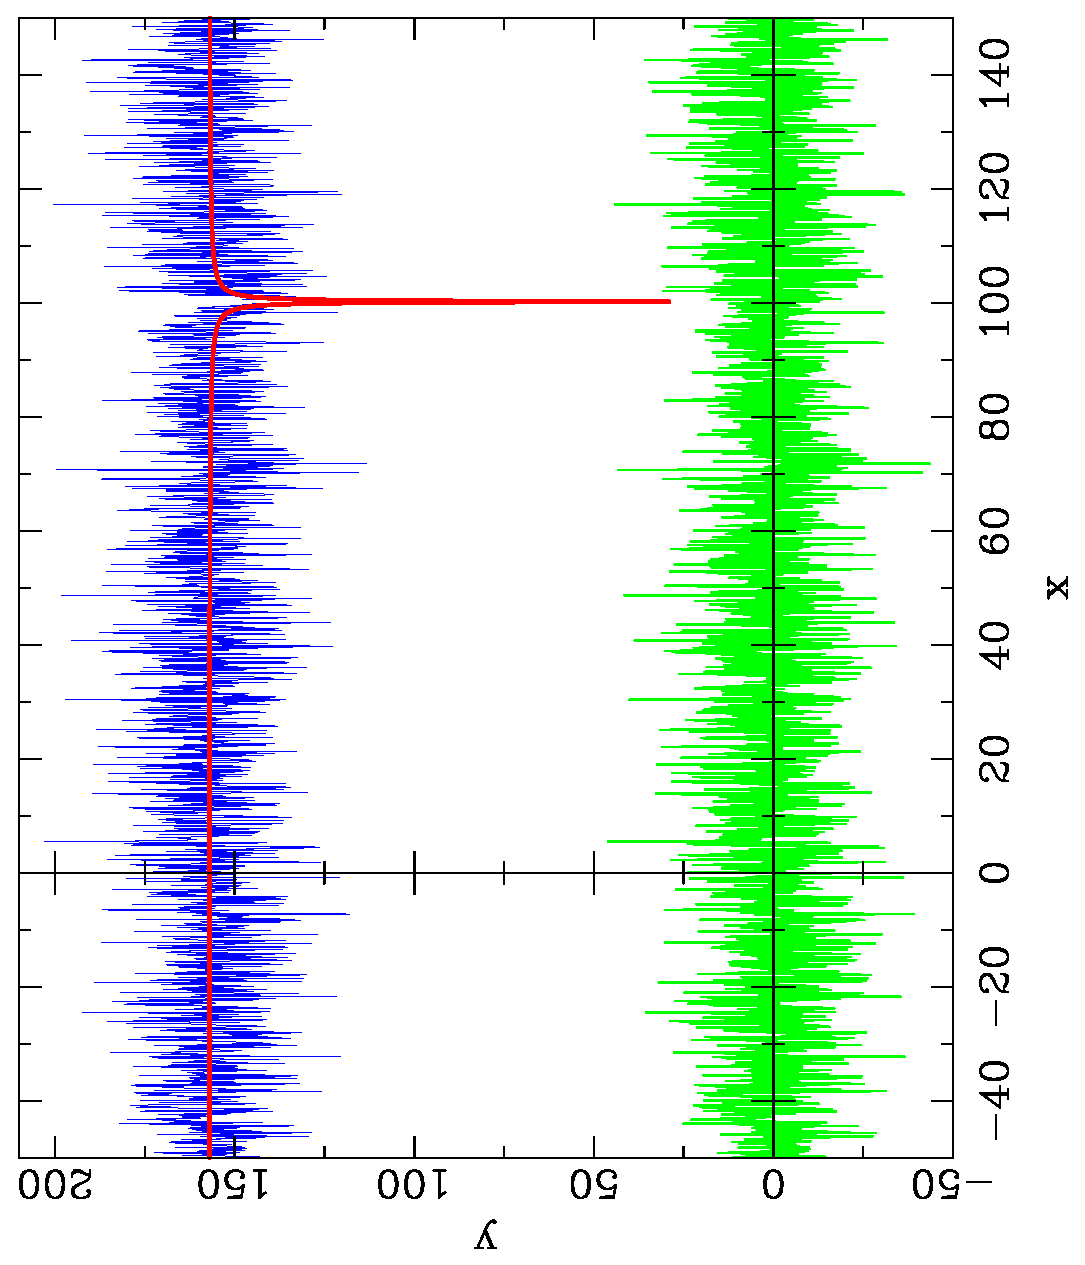
\includegraphics[angle=270,scale=0.45]{example.ideal.eps}
   \caption{Example data in comparison to the ideal function. The
    R-value between the observed and calculated function is 8.18\%.}
   \label{fexa-ideal}
\end{figure}

This data set proves to be a very hard challenge for any least squares
algorithm. Unless the starting values are very close to the actual
values, the least squares algorithm will not find the global minimum.
The very high noise level effectively prevents the algorithm from
finding the position of the minimum. Instead the R-value is minimized
by setting $P_{3}$ to the smallest positive value. At this level, the
width of the function is reduced to one point, if any. Furthermore, the
slope of the function is essentially zero for all x, and the position of
the minimum does not influence the R-value. The R-value is, however,
significantly above the R-value that is achieved for the ideal 
parameter values, show in Fig. \ref{fexa-ideal}.

To refine the function with \diffev, we need to define a couple of
items. These include:
\begin{itemize}
  \item Population size
  \item Limits, starting range etc. for the parameters $P_{i}$
  \item Values for refinement control variables
  \item location and names for files
\end{itemize}

The optimum size of a population is not always straightforward to
estimate. Since the minimum at $P_{1}$ is very narrow, a fairly 
large population size is advisable. A test shows that the population
should consist of approximately 40 members to ensure that the 
minimum is found.  The corresponding commands would be:
\begin{MacVerbatim}
  pop_n[1]   = 40
  pop_c[1]   = 40
  pop_gen[1] =  0
\end{MacVerbatim}
Here the number of members and children was set to the same value,
there is no fixed need to do so, unless the selection mode is set 
to compare a child with its immediate parent. With the last statement
the current generation number is set to zero. If a refinement is to 
be continued, the generation number can be set to the corresponding 
value.

The next group of definitions includes the number of parameters,
and then for each parameter a suitable name, hard boundaries, a
starting range and definitions how to handle parameter behavior 
at the hard boundary and in a local search.

In the current example, we have three parameters, all of which are 
floating numbers. None of the parameters has any absolute lower or
upper boundary imposed by external rules. Parameter $P_{3}$ must
not be equal to zero, this we will handle later as a constraint.
Sensible hard limits for the parameters could be:\\
\begin{tabular}{lp{2cm}p{2cm}p{8cm}}
     parameter & \raggedright{lower boundary}
               & \raggedright{upper boundary}
               & comment\\
     \hline
     1 &   0 & 200 & \raggedright{All data points are larger than zero.}
                     \tabularnewline
     2 & -50 & 150 & \raggedright{Minimum must be somewhere within the 
                                  observed x-range}
                     \tabularnewline
     3 &  -1 &  1  & \raggedright{Include zero to use constraints}
\end{tabular}
\\
\par 
If one has good estimates for the parameter values, these can be used 
to limit the initial spread of the population. A narrow spread of the
initial population around the expected final value will speed up the
convergence. Should these estimates prove to be wrong, however, the 
refinement will take extra long or may fail altogether. Here we will
not impose any prior knowledge on any of the parameters and use the
full range set by the hard boundaries.

During the initial refinement stages, the differences between the 
members will be large and chances are that the donor falls outside 
the allowed hard boundary interval. \Diffev corrects this situation by 
setting the violating parameter to a Gaussian distributed value 
with mean at the hard boundary. The respective half of the Gaussian
distribution that falls inside the boundary range is taken as valid
region. The user can set the sigma for this distribution and define
whether this sigma shall remain constant or be adapted during the
refinement. For parameters 1 and 2 we will set the initial sigma to
1, and for parameter 3 to 0.02. In later refinement cycles the
value of sigma can be adapted to a fraction of the total parameter 
spread, in our example to 0.2 of the parameter spread. 

Similarly, the sigma for a local search is fixed to starting values 
and adapted to a fraction of 0.01 of the total parameter spread.

For parameter 1 this would be set by the commands:
\begin{MacVerbatim}
   pop_name    1,height
   type real,1
   pop_xmin[1] =   0.0
   pop_xmax[1] = 200.0
   pop_smin[1] =   0.0
   pop_smax[1] = 200.0
   pop_sig [1] =   1.0
   pop_lsig[1] =   0.1
   adapt sigma , 1,0.2
   adapt lsigma, 1,0.01
\end{MacVerbatim}

As of version 5.16, \Diffev offers a shortened version of these 
commands with standardized values for the sigmas:
\begin{MacVerbatim}
   newparam height, 0.0, 200.0, 0.0, 200.0
\end{MacVerbatim}

If needed optional parameters can specify more details:
\begin{MacVerbatim}
   newparam height, 0.0, 200.0, 0.0, 200.0, init:keep
   newparam height, 0.0, 200.0, 0.0, 200.0, init:initialize
   newparam height, 0.0, 200.0, 0.0, 200.0, type:integer
   newparam height, 0.0, 200.0, 0.0, 200.0, type:real
\end{MacVerbatim}

This command assumes the {\it good} values sigma = 0.001 and 
local sigma = 0.0001 and will adapt the sigma to a population 
width of 0.2 and the local sigma to 0.02 of the population width.

The command assumes that the parameter is real valued unless the
optional parameter "type" is set to "integer".

Since parameter $P_{3}$ forms the denominator of Eq. \ref{eq-exa-arc},
its value must not be equal to zero. Check the function with a couple 
of different parameters, or simple mathematical analysis 
would show that the product $P_{3}~P_{1}$ must also be larger 
than zero to produce the observed dip. A clear lower limit for 
$P_{3}$ can, however, not be given. Therefore, $P_{3}$ was allowed 
in the interval [-1:1], and we just have to exclude a value of zero.

If the problem is difficult to solve, or if one wants to get a quick
estimate of one parameter, one can choose to refine just a subset. 
Since we only have three parameters, we will refine all at the same
time.

\begin{MacVerbatim}
   constrain p[3].ne.0.0
   refine     all
\end{MacVerbatim}

The next group of definitions concerns the control variables. \Diffev
offers the two basic variables, the scale factor, by which the difference
vector is multiplied, {\tt diff\_f[1]}, and the cross over probability
{\tt diff\_cr[1]}. Both are limited to the interval [0:1]. For this
refinement problem, the actual value of the cross over probability does
not matter, the scale factor should be closer to one to ensure 
successful refinement.

A variation of the basic algorithm allows to add the difference vector to 
any point along the line between parent and donor base.
In this problem, the location does not influence the refinement, and 
we choose the value of 1, which corresponds to the original 
algorithm. Also, the value of the local search probability does not
affect the search efficiency in this example, as long as its value is 
smaller than a value of roughly 0.3, and here it is set to zero.

\begin{MacVerbatim}
   diff_cr[1]  = 0.8
   diff_f[1]   = 0.81
   diff_k[1]   = 1.0
   diff_lo[1]  = 0.0
\end{MacVerbatim}

The next choice concerns selection of the donor. One can either choose 
the current best member as donor, or choose the donor at random. 
Here the donor is chosen at random. 

If the dependency of the R-value on the parameters is a reasonably 
smooth distribution without too many false minima, one can accelerate 
the convergence by taking the combined group of parents and children 
and to choose the best members to form the next set of parents. 
Here this is a good choice.

\begin{MacVerbatim}
   donor      random
   selection  best,all
\end{MacVerbatim}

Finally we need to define filenames for the trial files, the results
and the two log files. To keep the output nicely sorted, these files
are written into a subdirectory {\tt DIFFEV}.

\begin{MacVerbatim}
   trialfile  DIFFEV/Trials
   restrial   DIFFEV/Result
   logfile    DIFFEV/Parameter
   summary    DIFFEV/Summary
\end{MacVerbatim}

This concludes the basic setup. Prior to the main refinement loop, we
just have to generate the initial parameter sets, which is done by
the command {\tt initialize}, which does not take any parameters.
This command sets the current generation number to zero and writes
a first version of all trial files.

\begin{MacVerbatim}
   init
\end{MacVerbatim}

The main refinement follows, usually in a loop over several generations.
Within the loop, the {\tt system} command must be used to execute the 
slave program or programs that calculate the R-value. Once these are 
done, the {\tt compare} command reads all R-values, and generates the
next generation of trial values. It also updates the log files. For a 
fixed number of refinement cycles this could be a construction like:

\begin{MacVerbatim}
   do i[0]=1,40
     system ./arctan
     compare
   enddo
\end{MacVerbatim}

A loop with 40 cycles is executed, using the external program "./arctan"
to calculate the R-values. In a UNIX environment the leading "./" 
specifies that the program {\tt arctan} is found in the current 
directory. Without this specifier, the UNIX shell would search for 
the program in the directories specified by the value of your 
{\em PATH} variable. 

An indefinite loop that requires manual intervention could be:

\begin{MacVerbatim}
   variable integer, terminate
   terminate = -1
   fopen 1, CONTINUATION
   fput  1, terminate
   fclose 1
   do while(terminate.eq.-1)
      system ./arctan
     compare
     fopen 1, CONTINUATION
     fget  1, terminate
     fclose 1
  enddo
\end{MacVerbatim}

The macro initially sets the variable {\tt terminate} to "-1" and 
writes this to the file {\tt CONTINUATION}. The loop is executed
until the value of the variable is no longer "-1". At each cycle
the content of file {\tt CONTINUATION} is read into variable 
{\tt terminate}. Thus, the macro will stop, if you edit this file
and change the number stored within.

Finally, the following macro checks the R-value and reacts accordingly.
The commands in this macro were used to generate the performance 
tests in chapter \ref{diff}.

\begin{MacVerbatim}
  variable integer,cycle
  cycle = 0
  do
    system ./arctan
    compare
    cycle = cycle + 1
  enddo until (bestr[1].lt.0.0817830 .or. cycle.gt.100)
\end{MacVerbatim}

The loop is run indefinitely, until either the R-value has fallen
below a threshold, or until the number of cycles exceeds 100.

\begin{figure}
   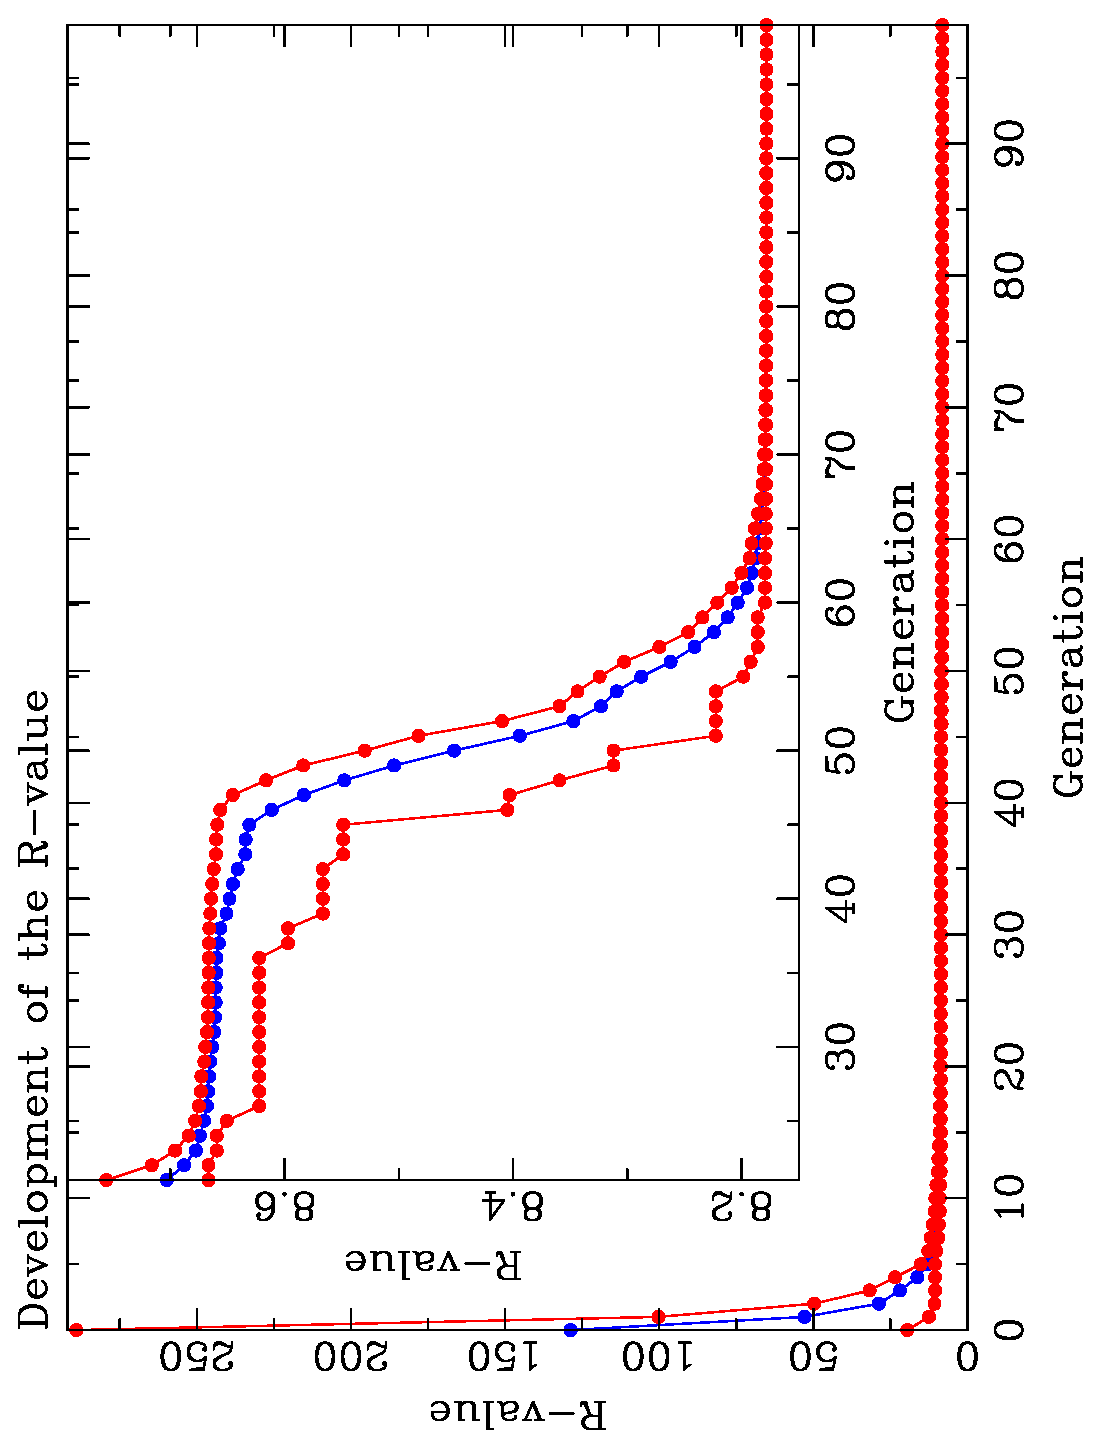
\includegraphics[angle=270,scale=0.45]{example.rval.eps}
   \caption{R-value as function of refinement generation. The Figure
            shows the best, worst R-value (red curves) and the average
            R-value (blue)}
   \label{fexa-rval}
\end{figure}

A typical refinement run is shown in Fig. \ref{fexa-rval}. The
refinement is set according to the control variables described in 
this section. Initially, the best and worst R-values quickly drop
to values around 9 to 12 \%. In these cycles, those parameter 
values that are really far off are eliminated. Thereafter, the 
real refinement starts. Up to generation 37 little change occurs.
At this stage, the first members have found the global minimum, 
and after generation 45 all members begin to converge into the 
global minimum, which is reached after generation 70. Thereafter,
no significant progress occurs.

\begin{figure}
   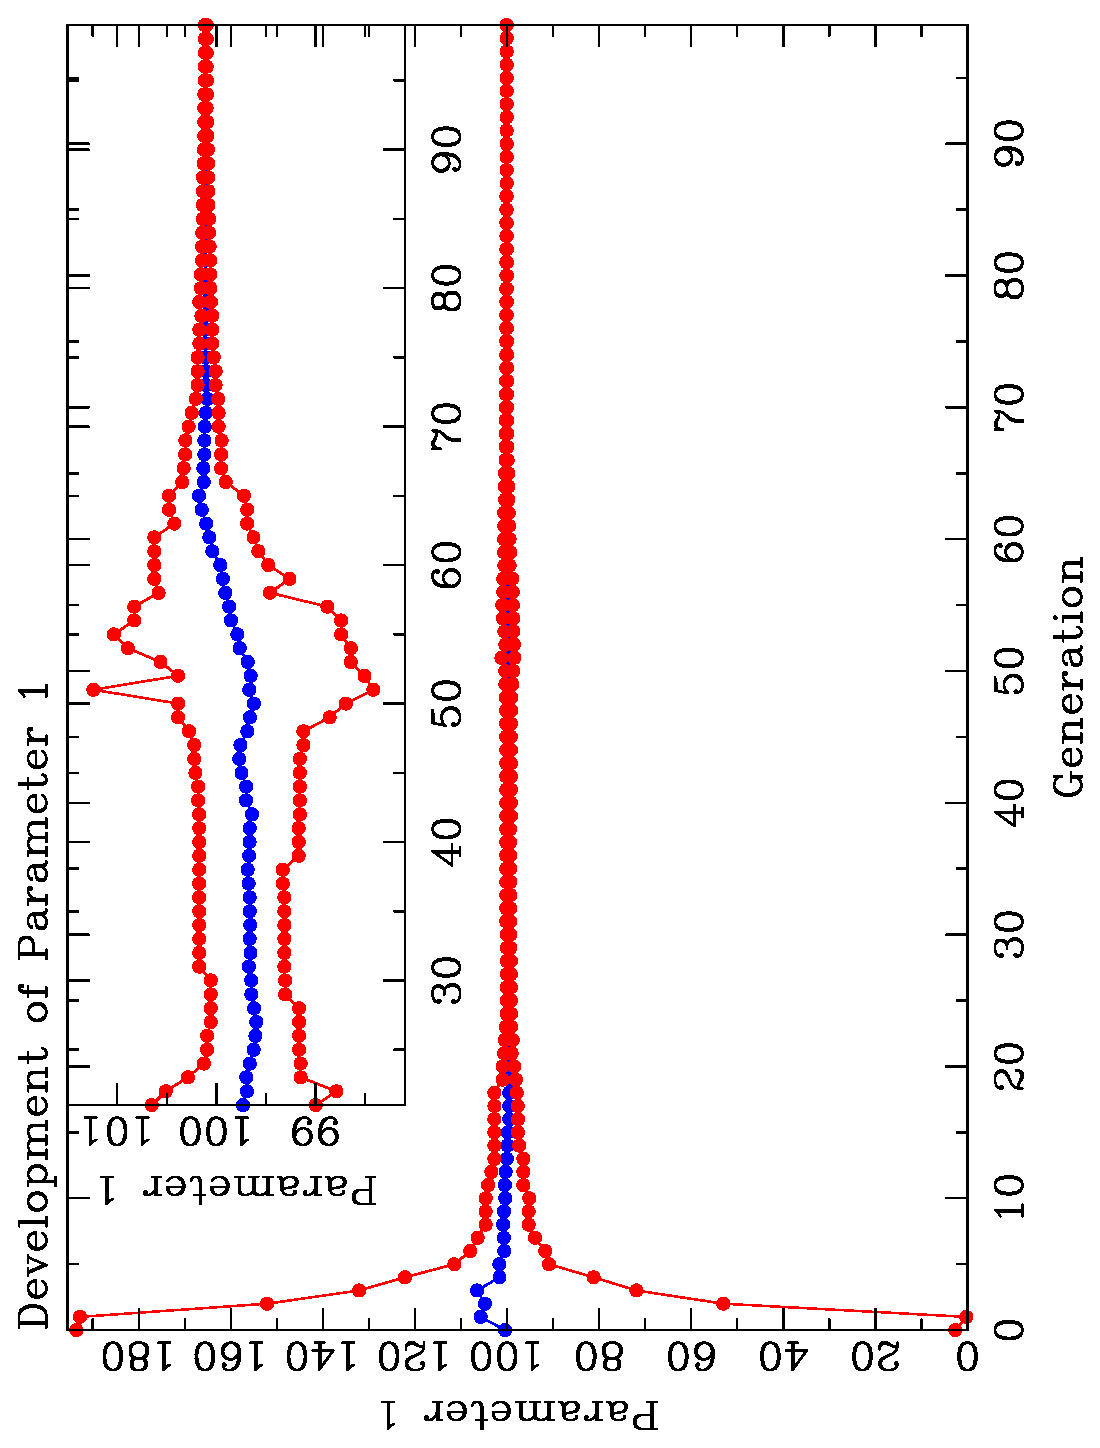
\includegraphics[angle=270,scale=0.45]{example.p1.eps}
   \caption{Parameter P1 as function of refinement generation. The Figure
            shows the best, worst R-value (red curves) and the average
            R-value (blue)}
   \label{fexa-p1}
\end{figure}

The main effect on the R-value is caused by the value of the parameter 
$P_{1}$, Fig. \ref{fexa-p1}, since this parameter lowers or raises 
the function over the 
whole x range. Accordingly, the refinement quickly finds a value close
to the right value. Notice that around generation 50, the parameter values
spread before the final value is found. It is around these generations
that all members find the global minimum and during the adjustment of
parameter $P_{3}$, the other parameters spread out for a few generations.

\begin{figure}
   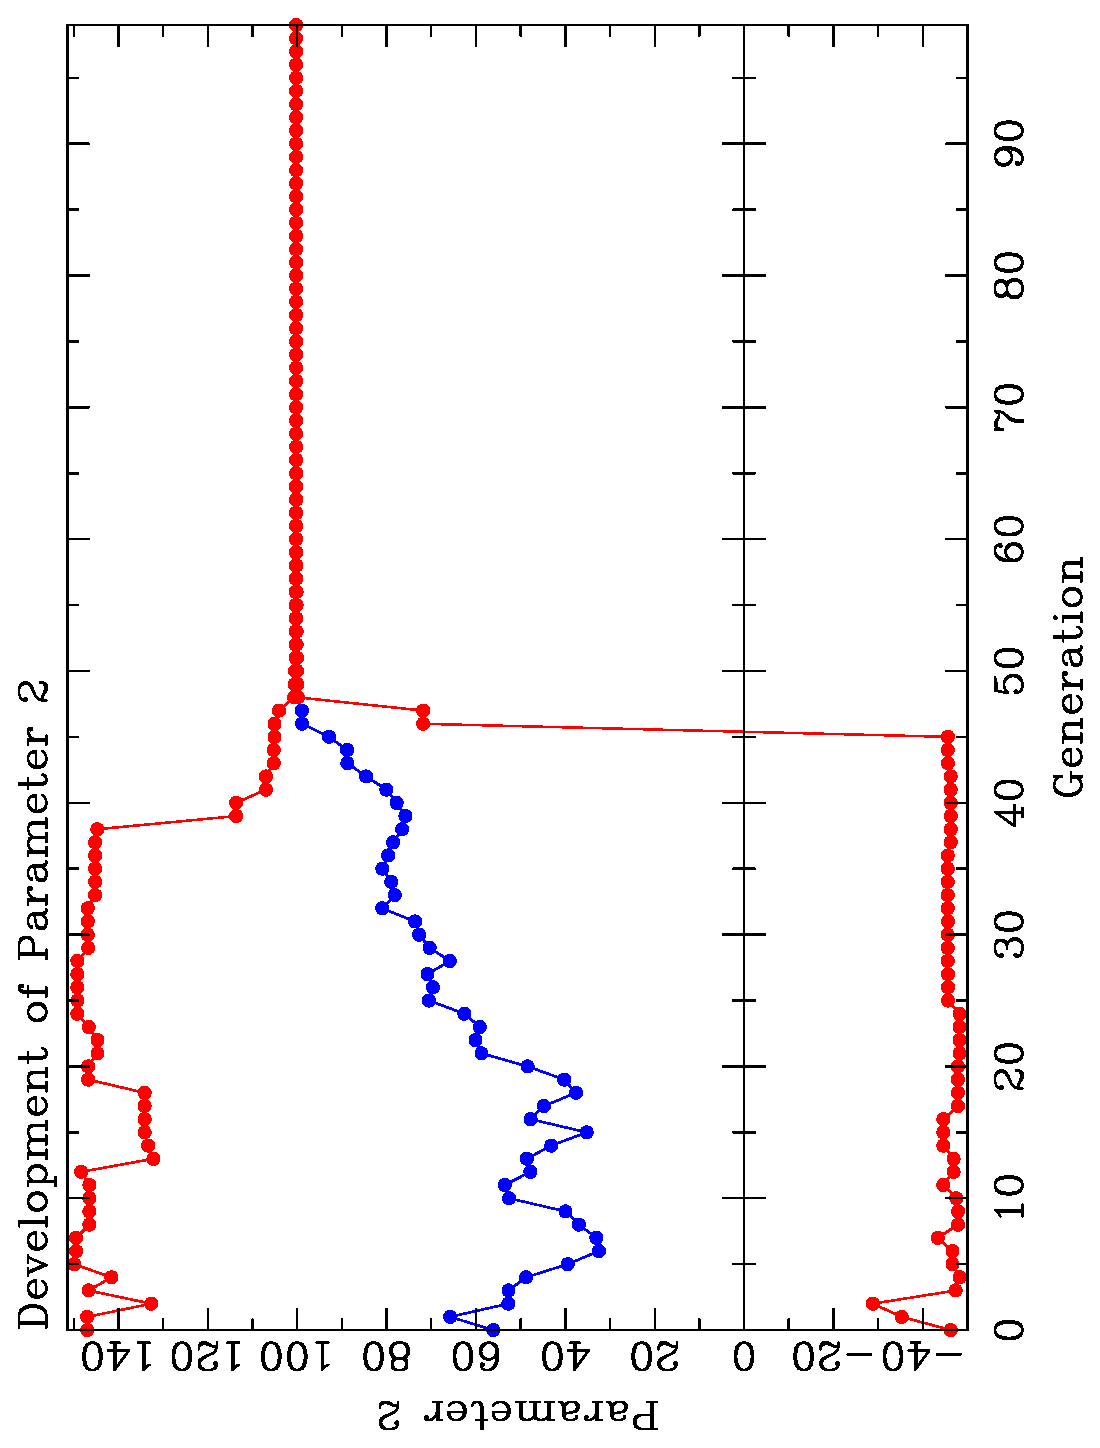
\includegraphics[angle=270,scale=0.45]{example.p2.eps}
   \caption{Parameter P2 as function of refinement generation. The Figure
            shows the best, worst R-value (red curves) and the average
            R-value (blue)}
   \label{fexa-p2}
\end{figure}

For the first roughly 15 generations, the value of parameter $P_{2}$,
Fg. \ref{fexa-p2}, hardly affects the R-value. As long as the position 
of the minimum is
not very close to the true value, its position hardly matters. 
From Generation 20 to 45 more and more members find the correct 
position.

\begin{figure}
   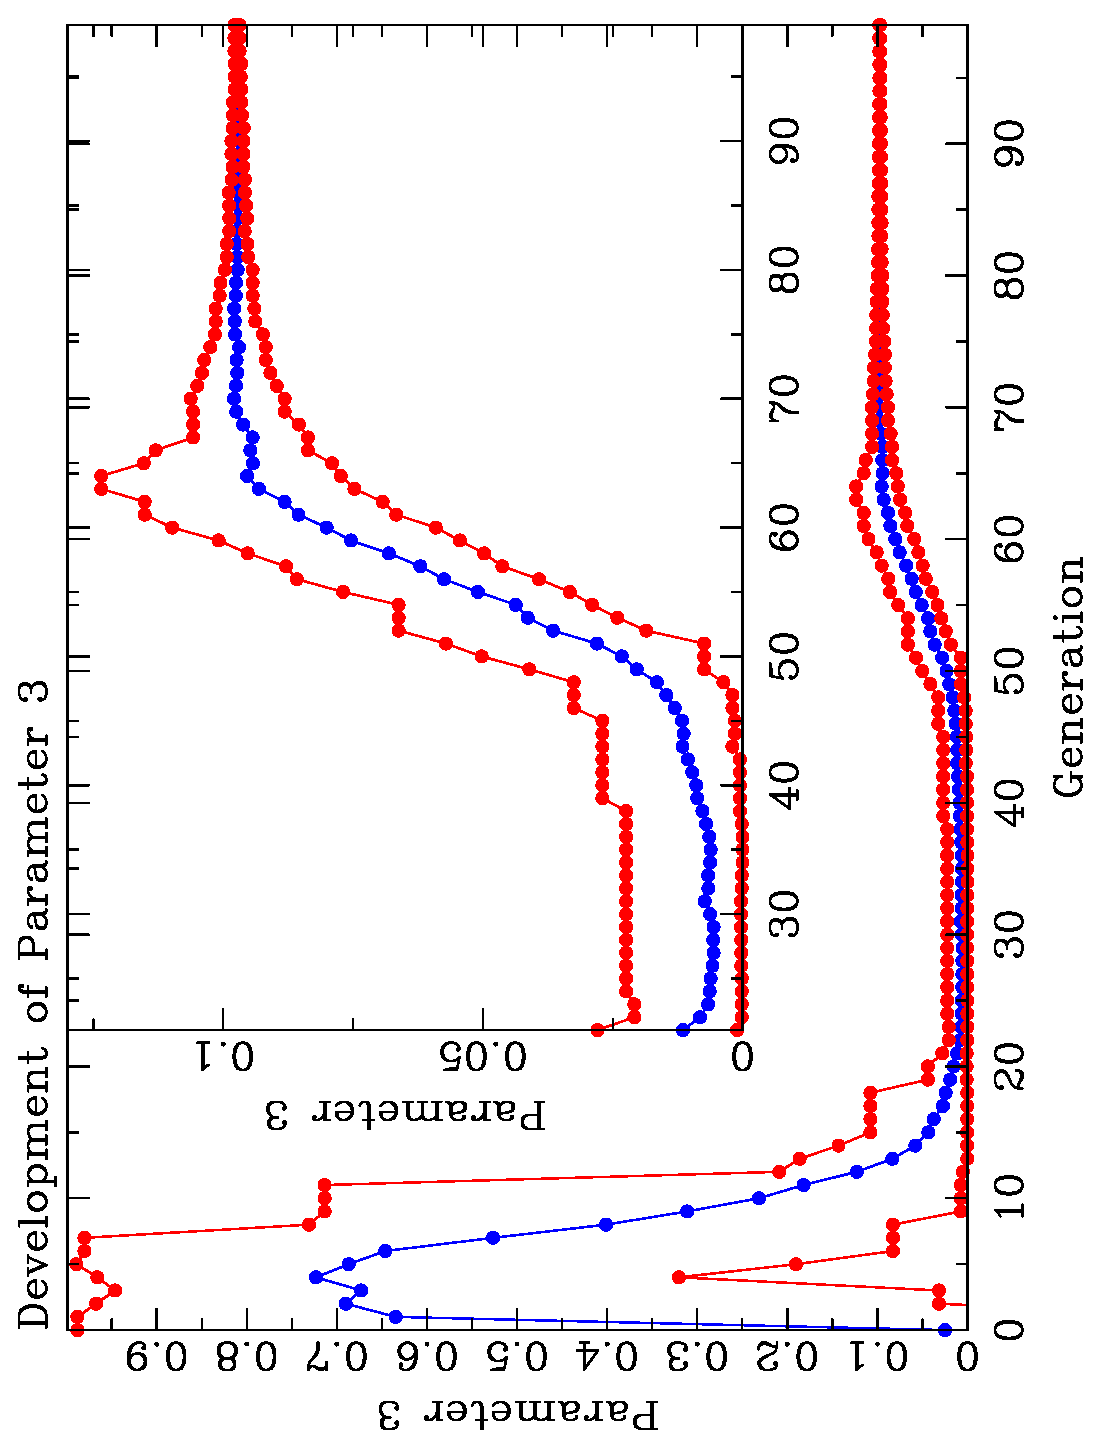
\includegraphics[angle=270,scale=0.45]{example.p3.eps}
   \caption{Parameter P3 as function of refinement generation. The Figure
            shows the best, worst R-value (red curves) and the average
            R-value (blue)}
   \label{fexa-p3}
\end{figure}

Parameter $P_{3}$, Fig. \ref{fexa-p3}, shows the most unusual refinement 
behavior. In the 
first few generation, all members with negative values of $P_{3}$ are
eliminated. The parameter then refines to values between zero and 0.02,
much lower than the true value. As long as the position of the minimum
is not found, lower R-values result if parameter $P_{3}$ is as close
to zero as possible. To get out of this local minimum, a large 
population size is required. Once the correct position is found,
parameter $P_{3}$ also refines to its correct value.

At this stage, the refinement is finished and the calculated curve 
is that of Fig. \ref{fexa-arc}. Admittedly, the difference between
the R-values around generations 30 at 8.65\% are not very 
significantly worse that the final R-value of 8.18\%. This is due to
the large amount of noise in the {\em experimental} data. 
These conditions were, however, chosen on purpose to illustrate
the ability of the differential evolutionary algorithm to jump out
of local minima, even under adverse conditions.

\section{Fixing, Releasing refinement parameters}

Most of the time, one will want to refine the parameters that have 
been defined and given a range with the {\tt newpara} command. 
This was done in the macro {\tt diffev\_setup.mac} in section
\ref{example}.

There are, of course, situations when you might want to fix one or
several parameters. This can be done with the \Diffev command
{\tt fix} that takes the form:

\begin{MacVerbatim}
  fix <Parameter_name>, <value>
  fix <Parameter_name>, best
\end{MacVerbatim}

The first command form fixes the parameter called {\tt Parameter\_name}
to the number given by {\tt value}. The second form  fixes the parameter 
to the value that correspond to the current best member in the population.

Instead of the parameter name, the parameter number can also be given, but
the preferred syntax would be to use the parameter name.

The {\tt fix} command sets the refine glag for the parameter off. The
command also sets the absolute and the starting boundaries to the 
parameter value. 

The complementary command to {\tt release} a fixed parameter takes the 
form:
\begin{MacVerbatim}
  release <Parameter_name>, range:<sigma>
\end{MacVerbatim}

This command initializes the parameter to a range {\tt current value $\pm$ 
sigma}. The lower and upper absolute parameter boundaries are fixed to
{\tt current value $\pm$ 3*sigma}. The refine flag is set to {\tt refine}.

To fine tune the {\tt release} command the following further optional 
parameter are available:
\begin{MacVerbatim}
   value:<setpoint>
   min:<pop_xmin>
   max:<pop_xmax>
   dismiss:<number>
\end{MacVerbatim}

The {\tt value} parameter serves to define a new setpoint for the parameter
insteiad of the current (fixed) value.  With {\tt min} and {\tt max} you 
have full control to define the lower and upper absolute parameter boundaries. 

Take as an exampe, the stacking fault parameter from the example in section
\ref{example}. It could be a good idea to constrain this parameter to a 
fixed value of 1.00 at the beginning of the refinement. This would correspond
to an ideal zincblende structure free of stacking faults. Later on the parameter 
might need to be refined. As the \Discus stacking fault parameter is fixed to a 
range 0 to 1, the release command is well off to set a new setpoint at a value 
somewehere between 0 and 1. If we take as an example a setpoint of 0.9, and a range
of 0.4, \Diffev would initialize the parameter in a range from 0.5 to 1.3. 
Furthermore, the absolute limits would be set to -1.1 and 2.1. Most of these
numbers are outside the physical limits of the \Discus stacking fault parameter.
Thus it is necessary to set the limits explicitly to 0.0 and 1.0 or other
values within the allowed range.

If a parameter is released, chances are, that the R-values of all children
are worse than the parents. In this case all trial parameters for the children 
would be ignored and \Diffev will take the parent values to generate the
next generation. In this case, all parent values for the parameter that we want
to release would revert back to the constant fixed value and the release would
be lost. To prevent this from happening, \Diffev offers the main command
{\tt dismiss} or the optional {\tt dismiss:} parameter at the {\tt release} 
command. The purpose is to assign to some of the parents an excessivly high 
R-value. This will be done to the worst members in the population and ensures
that for each of these members the child will have a lower R-value and will 
thus survive into the next generation. The {\tt dismiss:} parameter expects 
the number that signifies how many of the worst members shall be dismissed.
The number can be specified either as a constant value or an expression.
The allowed range is between 0 and the number of members in the population. 
With a value of "1", only the worst member is dismissed, with "2" the two
worst members and so on.
Otherwise the number can be given as keywords "all", "best" or "none".

\begin{tabular}{lp{12cm}}
     keyword & {Description} \\
     \hline
     0 & {No member of the population is dismissed} \\
         \hline
     n & {The worst "n" population members are dismissed} \\
         \hline
     all & All members are dismissed \\
         \hline
     best & All but the best member are dismissed \\
         \hline
     none & No member is dismissed, same as number 0 \\
         \hline
\end{tabular}


%------------------------------------------------------------------------

